\section{The LUX-ZEPLIN Detector}
\label{sec:lz_detector}
\par
The LUX-ZEPLIN (LZ) experiment is a second-generation direct detection dark matter experiment, named from it's predecessor LUX \cite{lux_ref}, and the ZEPLIN series of experiments which pioneered xenon phase detectors \cite{zeplin_3_ref}.
The LZ experiment is hosted at the Sanford Underground Research Facility (South Dakota, USA), at the 4850" level underground.


\par
The LZ experiment is a multi-detector system, which work together to increase the sensitivity to dark matter candidates.
LZ is comprised of three discrete detectors; a TPC, and two active veto-detectors.
A diagram of the detector systems is shown in \autoref{fig:LZ_Cut_CAD}.

\begin{figure}
    \centering
    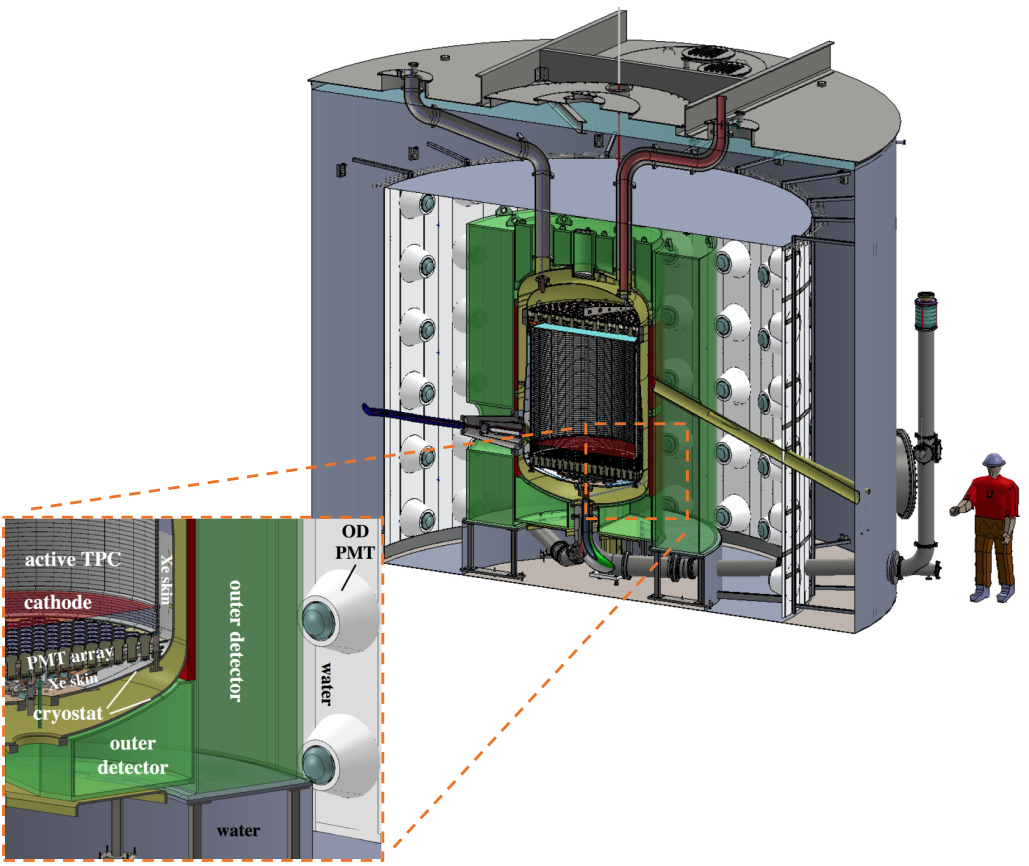
\includegraphics[width=\textwidth]{Figures/LZ/LZ_CAD_with_interactions.png}
    \caption{A schematic of the LZ detector systems as described in the Technical Design Review \cite{LZ_TechnicalDesignReview_ref}.
             Figure from \cite{LZ_TechnicalDesignReview_ref} using adaptation from \cite{LZ_Ibles_LZStats_Thesis_ref}.}
    \label{fig:LZ_Cut_CAD}
\end{figure}

\par
In the remainder of this chapter, the design and construction of the LZ experiment are detailed with particular emphasis on the TPC, Skin and OD which are relevant for the remainder of this thesis. 
It should be noted that the design is detailed in significant more detail in the Technical Design Review \cite{LZ_TechnicalDesignReview_ref}.

\subsection{Time Projection Chamber}
\label{sec:lz_tpc}
\par
At the core of LZ is a dual-phase (liquid and gas) Xenon TPC.
The schematic of the LZ TPC is shown in XXX.
Photons which are emitted inside of the TPC are detected by 494 Hamamatsu R11410-22 3-inch diameter PMTs, arranged into two arrays.
The first array contains 253 PMTs and is located at the top of the TPC in the GXe, looking down.
The second array, containing 241 PMTs and located at the bottom is immersed in the LXe looking up.
These PMTs were selected as they were developed with low levels of radioactivity and a high quantum efficiency at wavelengths around 175nm, the characteristic of LXe scintillation.
The arrangement of these PMT arrays is not identical, with the bottom array optimised for light collection of S1 signals, and the top array optimised for position reconstruction of S2 signals.
\par
The TPC contains three electrodes: a cathode at the bottom, a gate below the liquid surface and an anode in the gas phase, each of which are woven mesh grids \cite{lz_grids_ref}.
The walls of the TPC are enclosed by titanium rings encased in polytetrafluoroethylene (PTFE) panels - a highly reflective material (in excess of 97.3\% in LXe \cite{ptfe_lxe_reflectivity_ref}).
The titanium rings are connected by a resistor ladders.
These titanium rings act to shape the electric field, creating a vertical field across the entire active region such that any charge created in the active region will drift upwards through the liquid to the electroluminescence region.
\par
The TPC active region, which is defined as the volume between the cathode grid and the gate grid, is a cylinder of 1.46m diameter and height that contains 7-tonnes of Liquid Xenon.
This active region is a significant size increase compared to previous generation detectors such as LUX (250kg) \cite{lux_ref}, XENON1T (2.2-tonne) \cite{xenon1t_ref} and PandaX (500kg) \cite{pandax_ref}.
Other current generation Xenon TPC experiments include PandaX-4T (3.7-tonne) \cite{pandax_4t_ref} and XENONnT (5.9-tonne) \cite{xenonnt_projected_sensitivty_ref}, with both having recently published results from first runs \cite{pandax_4t_sr1_ref,xenonnt_sr1_er_ref}. 
\par
The electroluminescence region is defined as the distance from the surface of the LXe to the anode grid, an 8mm distance.
The distance between the gate grid and the anode grid is 13mm.
In the region, the electric field can reach 10 kV/cm.
This is typically referred to as the extraction field.
The electric field in the active region can reach 310 V/cm when applying an operating voltage of -50keV to the cathode.
\par
Below the cathode is a fourth grid which acts to shield the bottom array PMTs from the electric field.
Between this grid and the cathode is a reverse-field region (RFR), where the ionisation from interactions cannot be detected.


\subsection{Veto Detectors}
\label{sec:lz_veto_detectors}
\par
In addition to the TPC, the LZ experiment makes use of two additional detectors.
Neither of these are designed to directly detector dark matter, but rather to act to improve the sensitivity of the TPC by identifying events which would otherwise impact the TPCs ability to detector dark matter via anti-coincidence.

\par
Firstly, surrounding the TPC is a layer of LXe referred to as the Xenon Skin, or Skin detector.
This region of LXe has to exist due to the geometrical challenge of placing the TPC inside of a cryovessel.
As such it has been made active by 38 Hamamatsu R8778 2-inch PMTs in the barrel and bottom dome and 93 R8520 1-inch PMTs in the top barrel region.
Similarly to the TPC, the ICV inner-wall has been coated with PTFE, but is optically de-coupled from the TPC.

\par
Outside of the OCV, the second veto detector is the Outer Detector (OD).
This is made up of a number of acrylic tanks which contain a liquid scintillator doped with gadolinium (GdLS).



\autoref{fig:LZ_Veto_Principle}

The OD is described in more detail in \autoref{chapter:lz_outer_detector}.

\begin{figure}
    \centering
    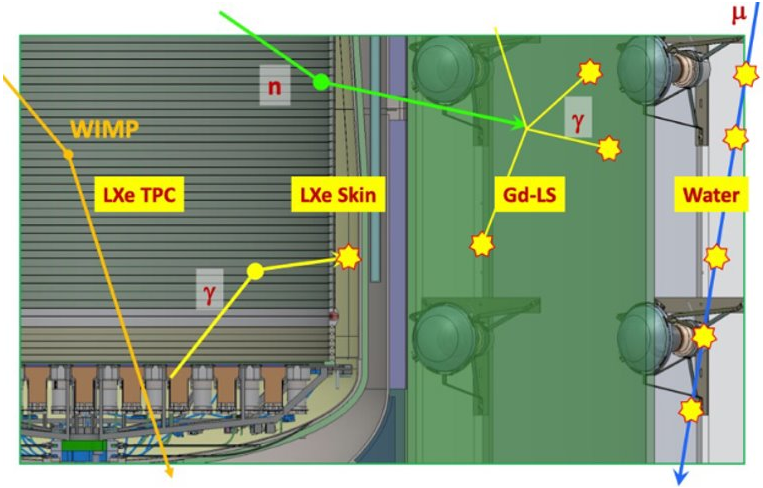
\includegraphics[width=0.75\textwidth]{Figures/LZ/lz_veto_plan.png}
    \caption{Depiction of operating principle of the veto detectors and the particles that they are designed to veto.}
    \label{fig:LZ_Veto_Principle}
\end{figure}


\subsection{OD}
\par
Surrounding OCV is the outer-detector (OD).
It consists of 10-segments of acrylic tanks (something about UV), which fit around the OCV as shown in Figure XXX.
Together these provide near 4$\pi$ coverage about the OCV.

\par
The OD tanks are filled with a linear akylbenze (LAB) doped with 0.1\% natural Gadolinium (by mass) - which together are refereed to as the Gadolinium Liquid Scintillator (GdLS).



\par



\subsubsection{Design Changes}
\par
During the installation phase of the Acrylic tanks about the OCV, the curvature of the top Acrylic tanks were significantly different to that of the OCV, as such, the top 2 acrylic tanks could not be placed around the 

\par


\subsection{Water}

\subsection{Underground}

\subsection{Backgrounds}

\subsection{Calibrations}
\par
In order for the above experiment to work and have understandable results, a set of calibrations are required to characterise the; energy scale, energy threshold and detection efficiency.
In this section the calibration systems are explained, along with the different sources that are deployable.
A summary of the sources used prior to SR1 are shown in Table XXX. 
Additional sources planed are outlined in the LZ Technical Design Review \cite{LZ_TechnicalDesignReview_ref}

\begin{table}[!htbp]
    \centering
    \begin{tabular}{c|c|c|c}
    \hline
    Isotope       & Interacting particle         & Purpose                    & Deployment \\
    \hline
    ${}^{83m}Kr $ & beta/gamma, 32.1 keV/9.4 keV & TPC (x,y,z)                & Internal  \\
    ${}^{131m}Xe$ & 164 keV gamma                & TPC (x,y,z), Xe skin       & Internal  \\ 
    ${}^{220}Rn $ & various alphas               & xenon skin                 & Internal  \\
    $AmLi       $ & (alpha, n)                   & NR band                    & CSD       \\
    ${}^{252}Cf $ & spontaneous fission          & NR efficiency              & CSD       \\
    ${}^{57}Co  $ & 122 keV gamma                & Xe skin threshold          & CSD       \\
    ${}^{228}Th $ & 2.615 MeV gamma              & OD energy scale            & CSD       \\
    ${}^{22}Na  $ & back-to-back 511 keV gamma’s & TPC and OD sync            & CSD       \\
    ${}^{88}Y Be$ & 152 keV neutron low-energy   & NR response                & External  \\
    $DD         $ & 2,450 keV neutron            & NR light and charge yields & External  \\
    $DD         $ & 272 keV neutron              & NR light and charge yields & External
    \end{tabular}
    \caption{LZ calibration sources that were used for calibration prior to the first science run along with the calibration purpose and deployment method. Table adapted from \cite{LZ_TechnicalDesignReview_ref}.}
    \label{tab:LZ_Used_Calibration_Sources}
\end{table}


\subsubsection{Internal}
\par

\subsubsection{Calibration Source Tubes}
\par

\subsubsection{External}
\par
External sources are sources which are outside of the OCV.

\section{Detector Status}
\par
During this thesis, the construction of the LZ experiment was completed, followed by a successful commissioning and calibration phase.
The first Science Run concluded April 2022 with the first result for the WIMP search announced June 2022.
The detector is currently undergoing Pre-SR2 upgrades, with SR2 due to commence September 2022.

